\documentclass{article}
\usepackage{graphicx}
\usepackage{float}

\begin{document}
\title{Study of activities on Amcrest View Camera}
\author{Abhinav Narain}
\section{Result}
Classification of three different activities was attempted with almost 90\% accuracy on Amcrest camera.
\begin{itemize}
\item Camera is idle (after reboot)
\item Camera is recording data when instructed by mobile app
\item Camera is streaming data when instructed by mobile app and moving the camera directions
\end{itemize}
\begin{figure}[H]
\centering
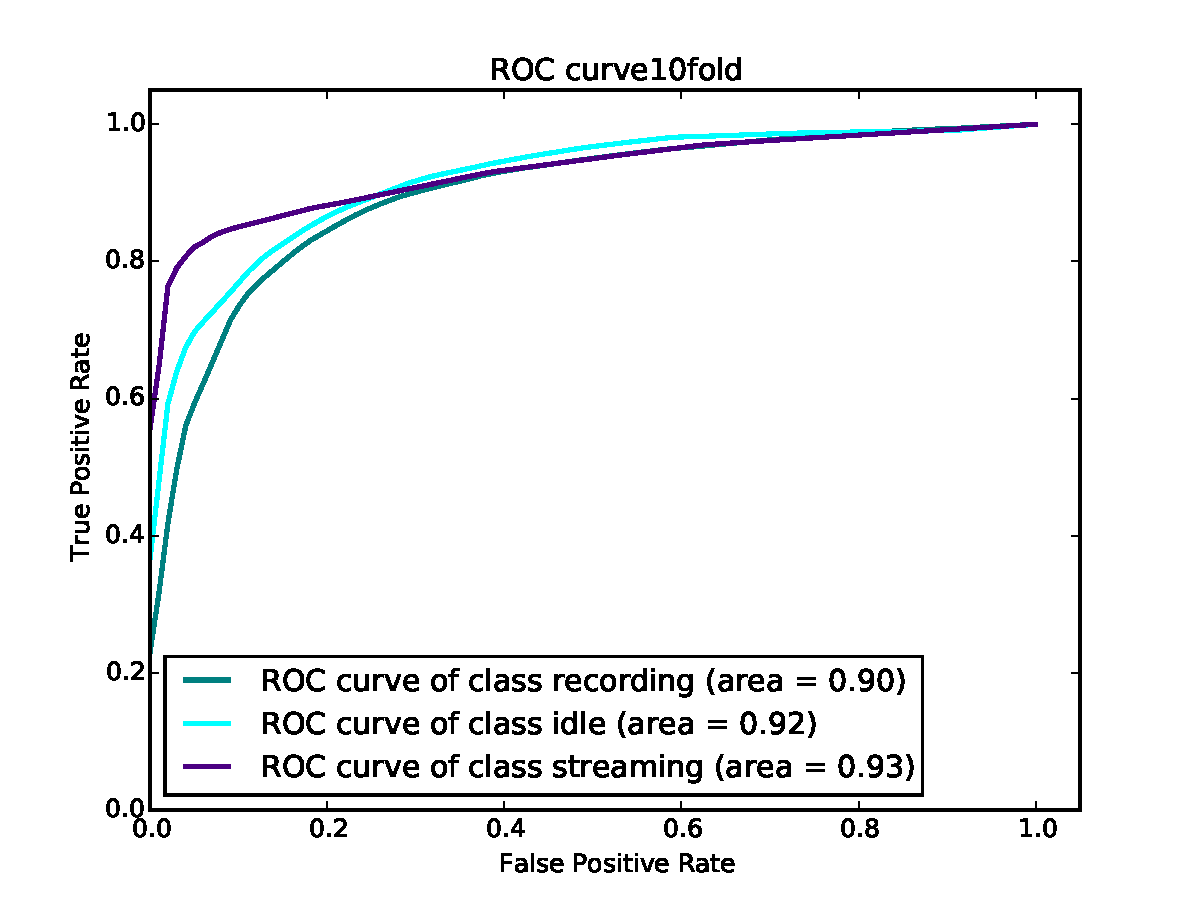
\includegraphics[width=\textwidth]{camera_plots/randfor_cAcD_roc_mult_haar.pdf}
\caption{ROC curve for classification between activities using Random Forest classifier}
\label{fig:roc}
\end{figure}

\section{Spectrograms of EMI activity of Amcrest View Camera}
\begin{figure}[H]
\centering
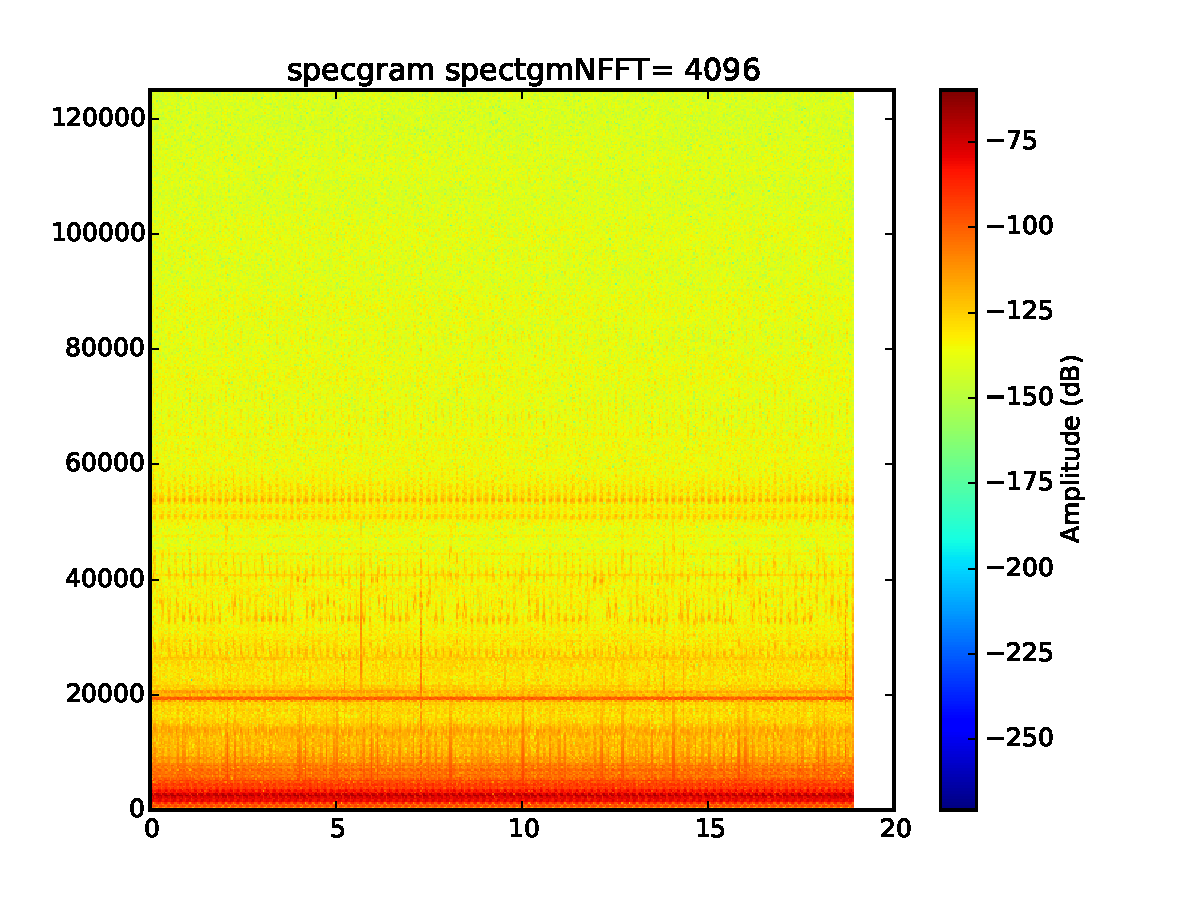
\includegraphics[width=\textwidth]{camera_plots/bandpass_decimate/decim_idle_500K_cam_4096_clipped.pdf}
\caption{The device is not instructed to do any function and is idle after boot}
\label{fig:idle}
\end{figure}

\begin{figure}[H]
\centering
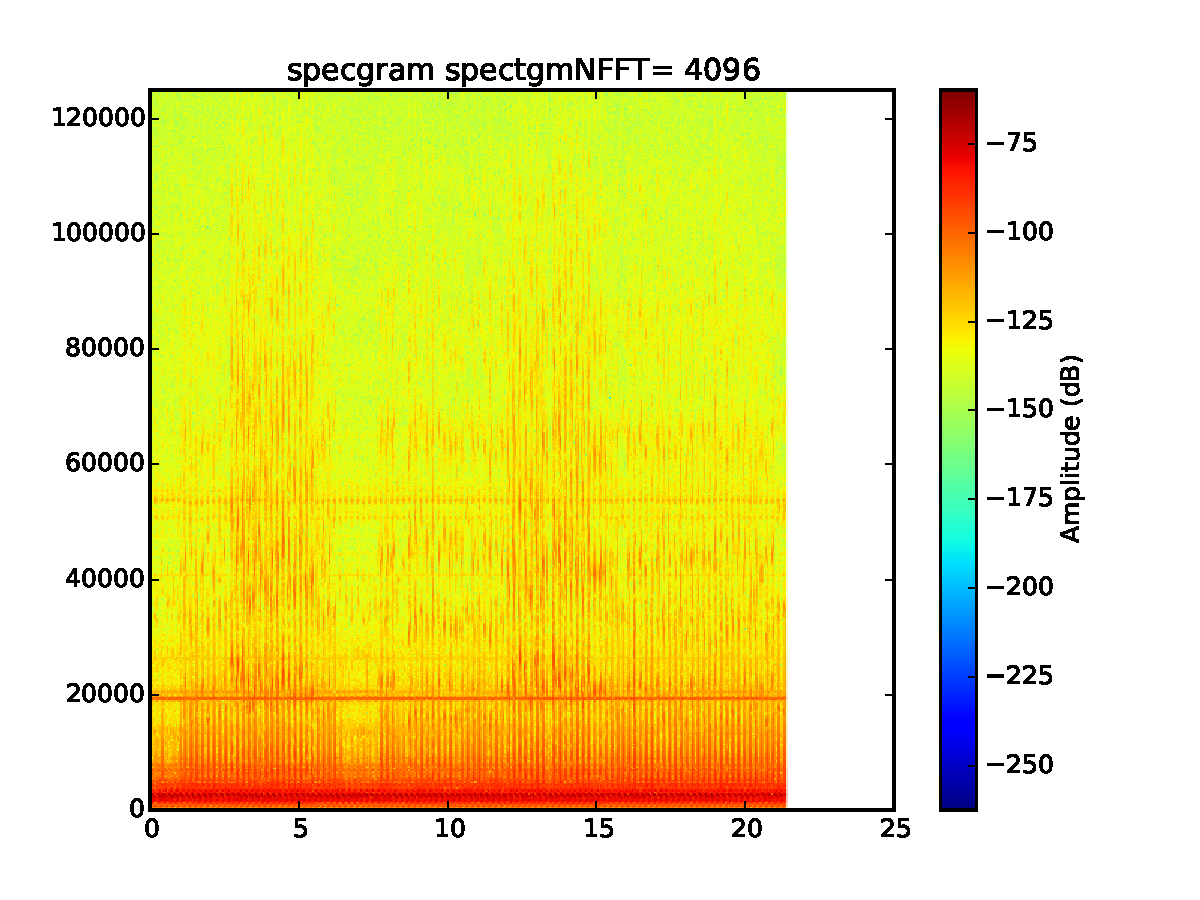
\includegraphics[width=\textwidth]{camera_plots/bandpass_decimate/decim_stream_500K_cam_4096_clipped.pdf}
\caption{The devices is streaming a video while one moves around the camera directions}
\label{fig:stream}
\end{figure}

\begin{figure}[H]
\centering
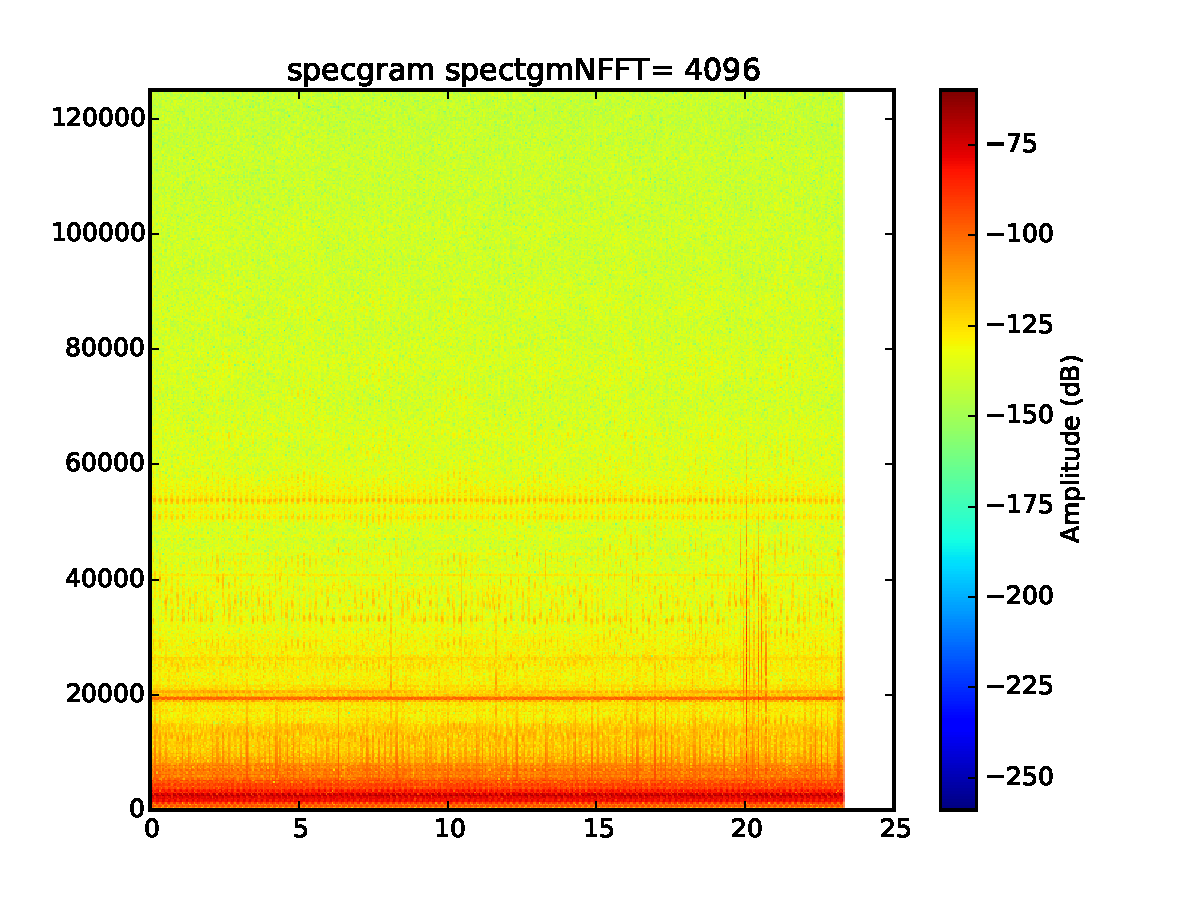
\includegraphics[width=\textwidth]{camera_plots/bandpass_decimate/decim_rec_500K_cam_4096_clipped.pdf}
\caption{The device is recording a video, instructed using a mobile app}
\label{fig:record}
\end{figure}

\begin{figure}[H]
\centering
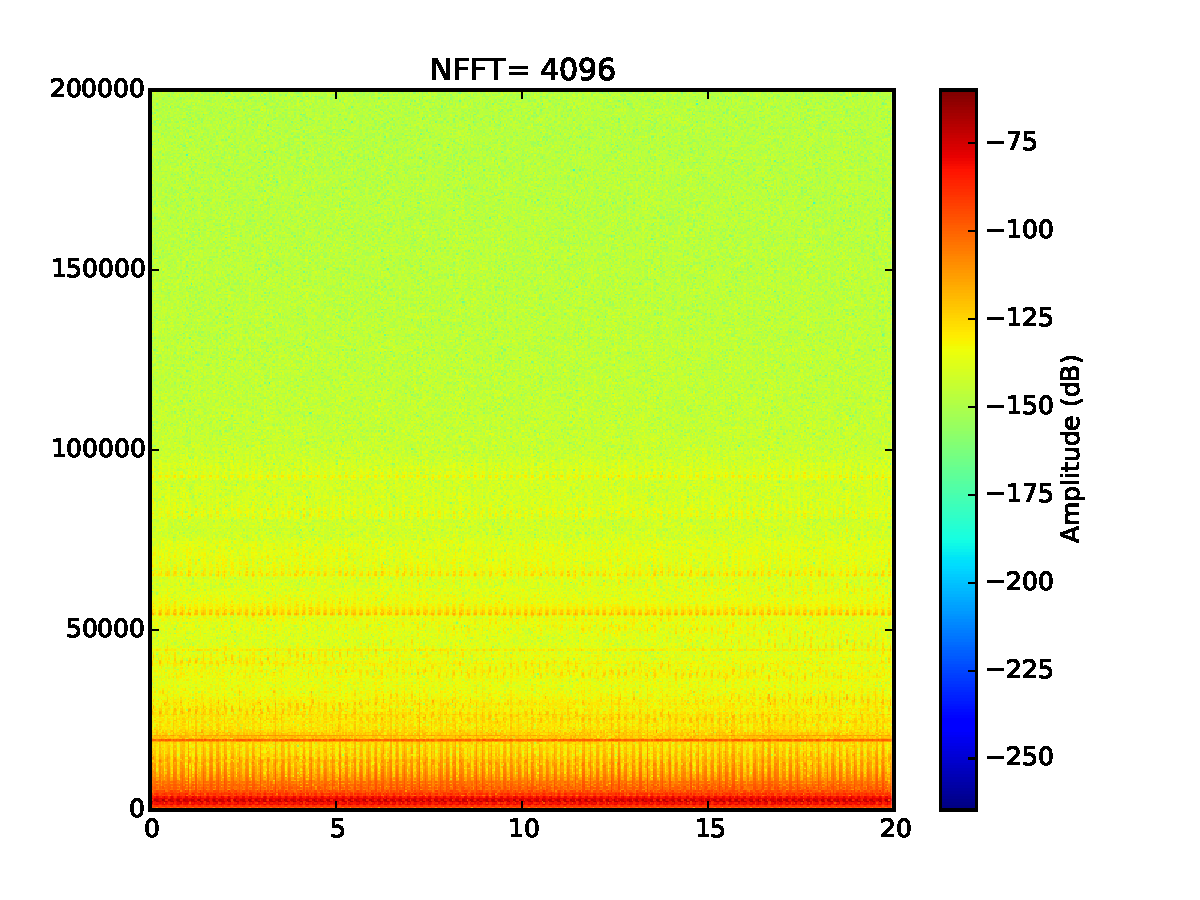
\includegraphics[width=\textwidth]{camera_plots/cam_snapshot_4096_clipped.pdf}
\caption{The device captured photographs at random times. No spikes were registered in spectrogram}
\label{fig:record}
\end{figure}





\end{document}
